% \section{Lined Arbitrage}
% \label{sec:line_arb}
% \begin{figure*}
%     \centering
%     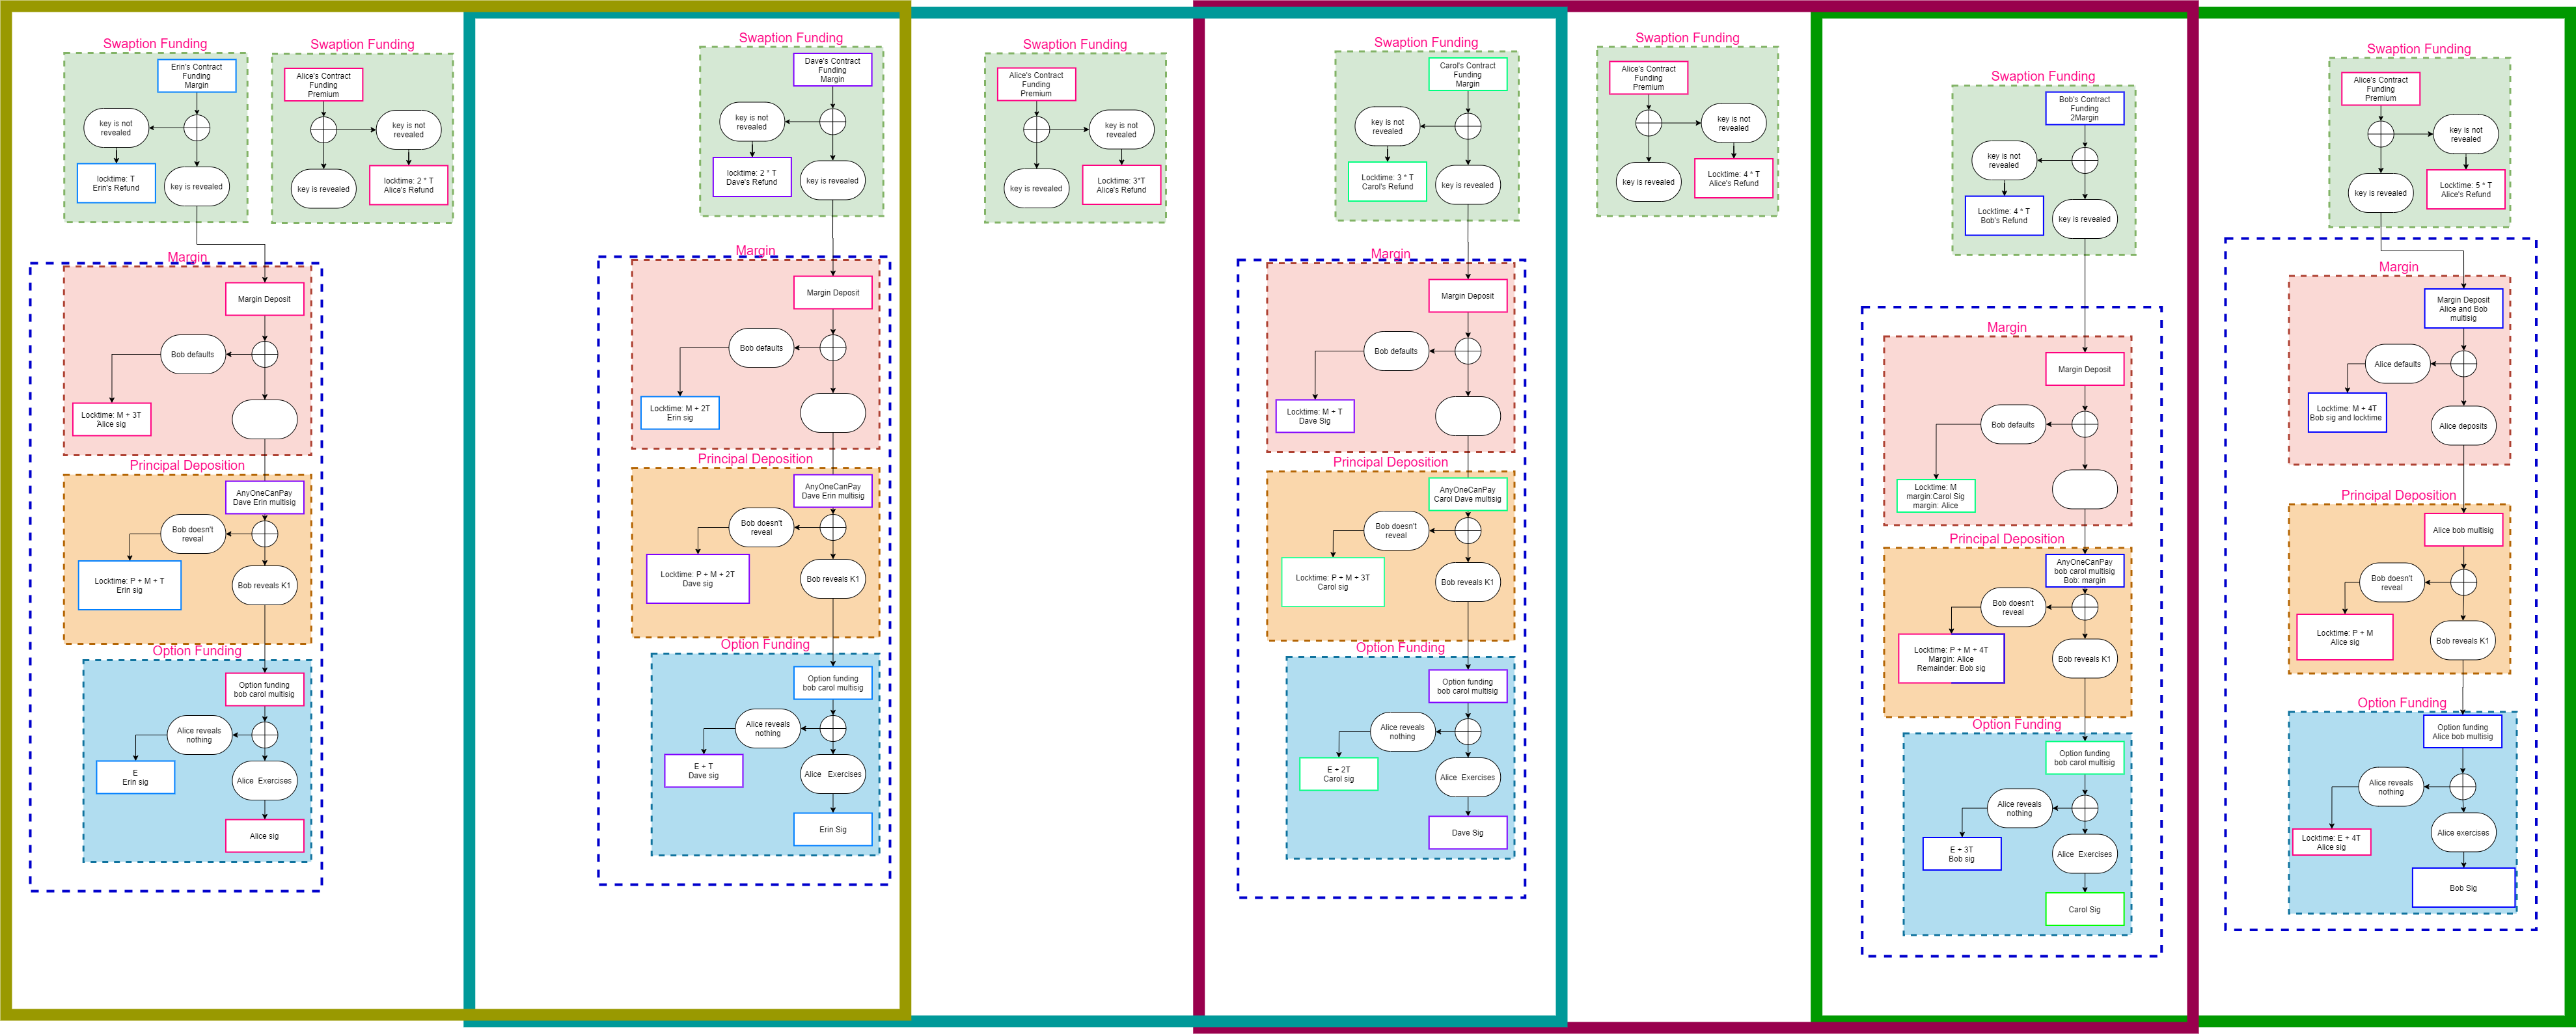
\includegraphics[width=\textwidth]{figures/lined-arbitrage.png}
%     \caption{Example of an arbitrage, where Alice owns all Acoins primarily needed.}
%     \label{fig:line_arb}
% \end{figure*}



% Imagine our example of arbitrge to be like: Alice does own enough Acoins, so she does not need to use Erin's Acoins and form a loop. Instead, she form an arbitrage in shape of a line, starting from swaption between Alice and Bob and ending in swpation between Dave and Erin. Fig ~\ref{fig:line_arb} shows this example. Note that in the normal instances of {\it Early Deposition} swaptions there is no Principal Deposition stage. But in this use case we have to add this stage for consistency between hash locks of different assets. Now pay attention to the four phases of this arbitrage:

% \begin{itemize}
%     \item \textbf{Contract Funding}: Alice starts her contract with other parties simultaneously, by sharing the funding transaction with them. Then she decides to reveal \Aone key or not. If she does, all the swaptions go to the next stage. The locktimes are set descending so that Alice can not cheat. In fact, Alice has to reveal \Aone before T, the minimum locktime among all swaptions, since otherwise at least one of them has expired and the entire arbitrage is not plausible any more. Note that if any of the funding stages fail, the entire arbitrage fails.
    
%     \item \textbf{Principal Deposition}: In this stage, every one has to deposit their principal. All swaptions except for the first one, are {\it Early Deposition} swaptions so their locktimes are ascending. The first swaption's locktimes are descending, though. Possible scenarios: 
%     \begin{itemize}
%         \item One of the parties defaults. In this case, all parties after the defaulter also default. Hence, the first defaulter looses his margin and  all the other parties transfer their margin with the next party in the line.
%         \item All parties deposit their principal and go to the next stage.
        
%     \end{itemize}
%     \fatemeC{The M locktime is assumed to be larger than the maximum time in the previous stage ($M > 5T$) so that there would not be any conflicts between stages.}
    
%     \item \textbf{Leader Lock}:The locktimes in the first swaption are ascending and in the rest of swaptions are descending. The reason is that in the first one Bob holds the \keyone key and in other ones Alice holds it. Note that Bob has the M + P + 3T locktime but in fact he has to reveal \keyone key before M + P, because otherwise Alice defaults and Bob loses his margin. parties take back their own money. By arranging timelocks in this way, no portion of parties can cheat on others by cooperating. Possible scenarios:
    
%     \begin{itemize}
%         \item Bob defaults. he looses one of his margins as discussed in {\it Late Deposition} swaption, while other
%         \item Bob reveals \keyone key by broadcasting Alice's option funding transaction. Then Alice broadcasts the Erin's Option Funding transaction, and other opponents do the same respectively. And we go to next stage. If any of them does not do this, the only one who looses money is that party.
%     \end{itemize}
%     \ahC{is it clear and okay or not? We can mention that all of the swaptions in the point of view of other opponent than Alice is just like an instance of Meta Swaption, accordingly no body can cheat by cooperation on others}
    
%     \item \textbf{Option Funding}: It is time for Alice to use her option. The locktimes are descending in all swaptions because in all of them Alice is the secret holder. Alice reveals \Atwo key by broadcasting the final transaction in the swaption with Erin. Then other parties broadcast their own related transactions in order and the arbitrage is executed. 
% \end{itemize}

% \subsection{Margined Arbitrage: Looped}
% \label{sec:margined_arb}


% \begin{figure*}
%     \centering
%     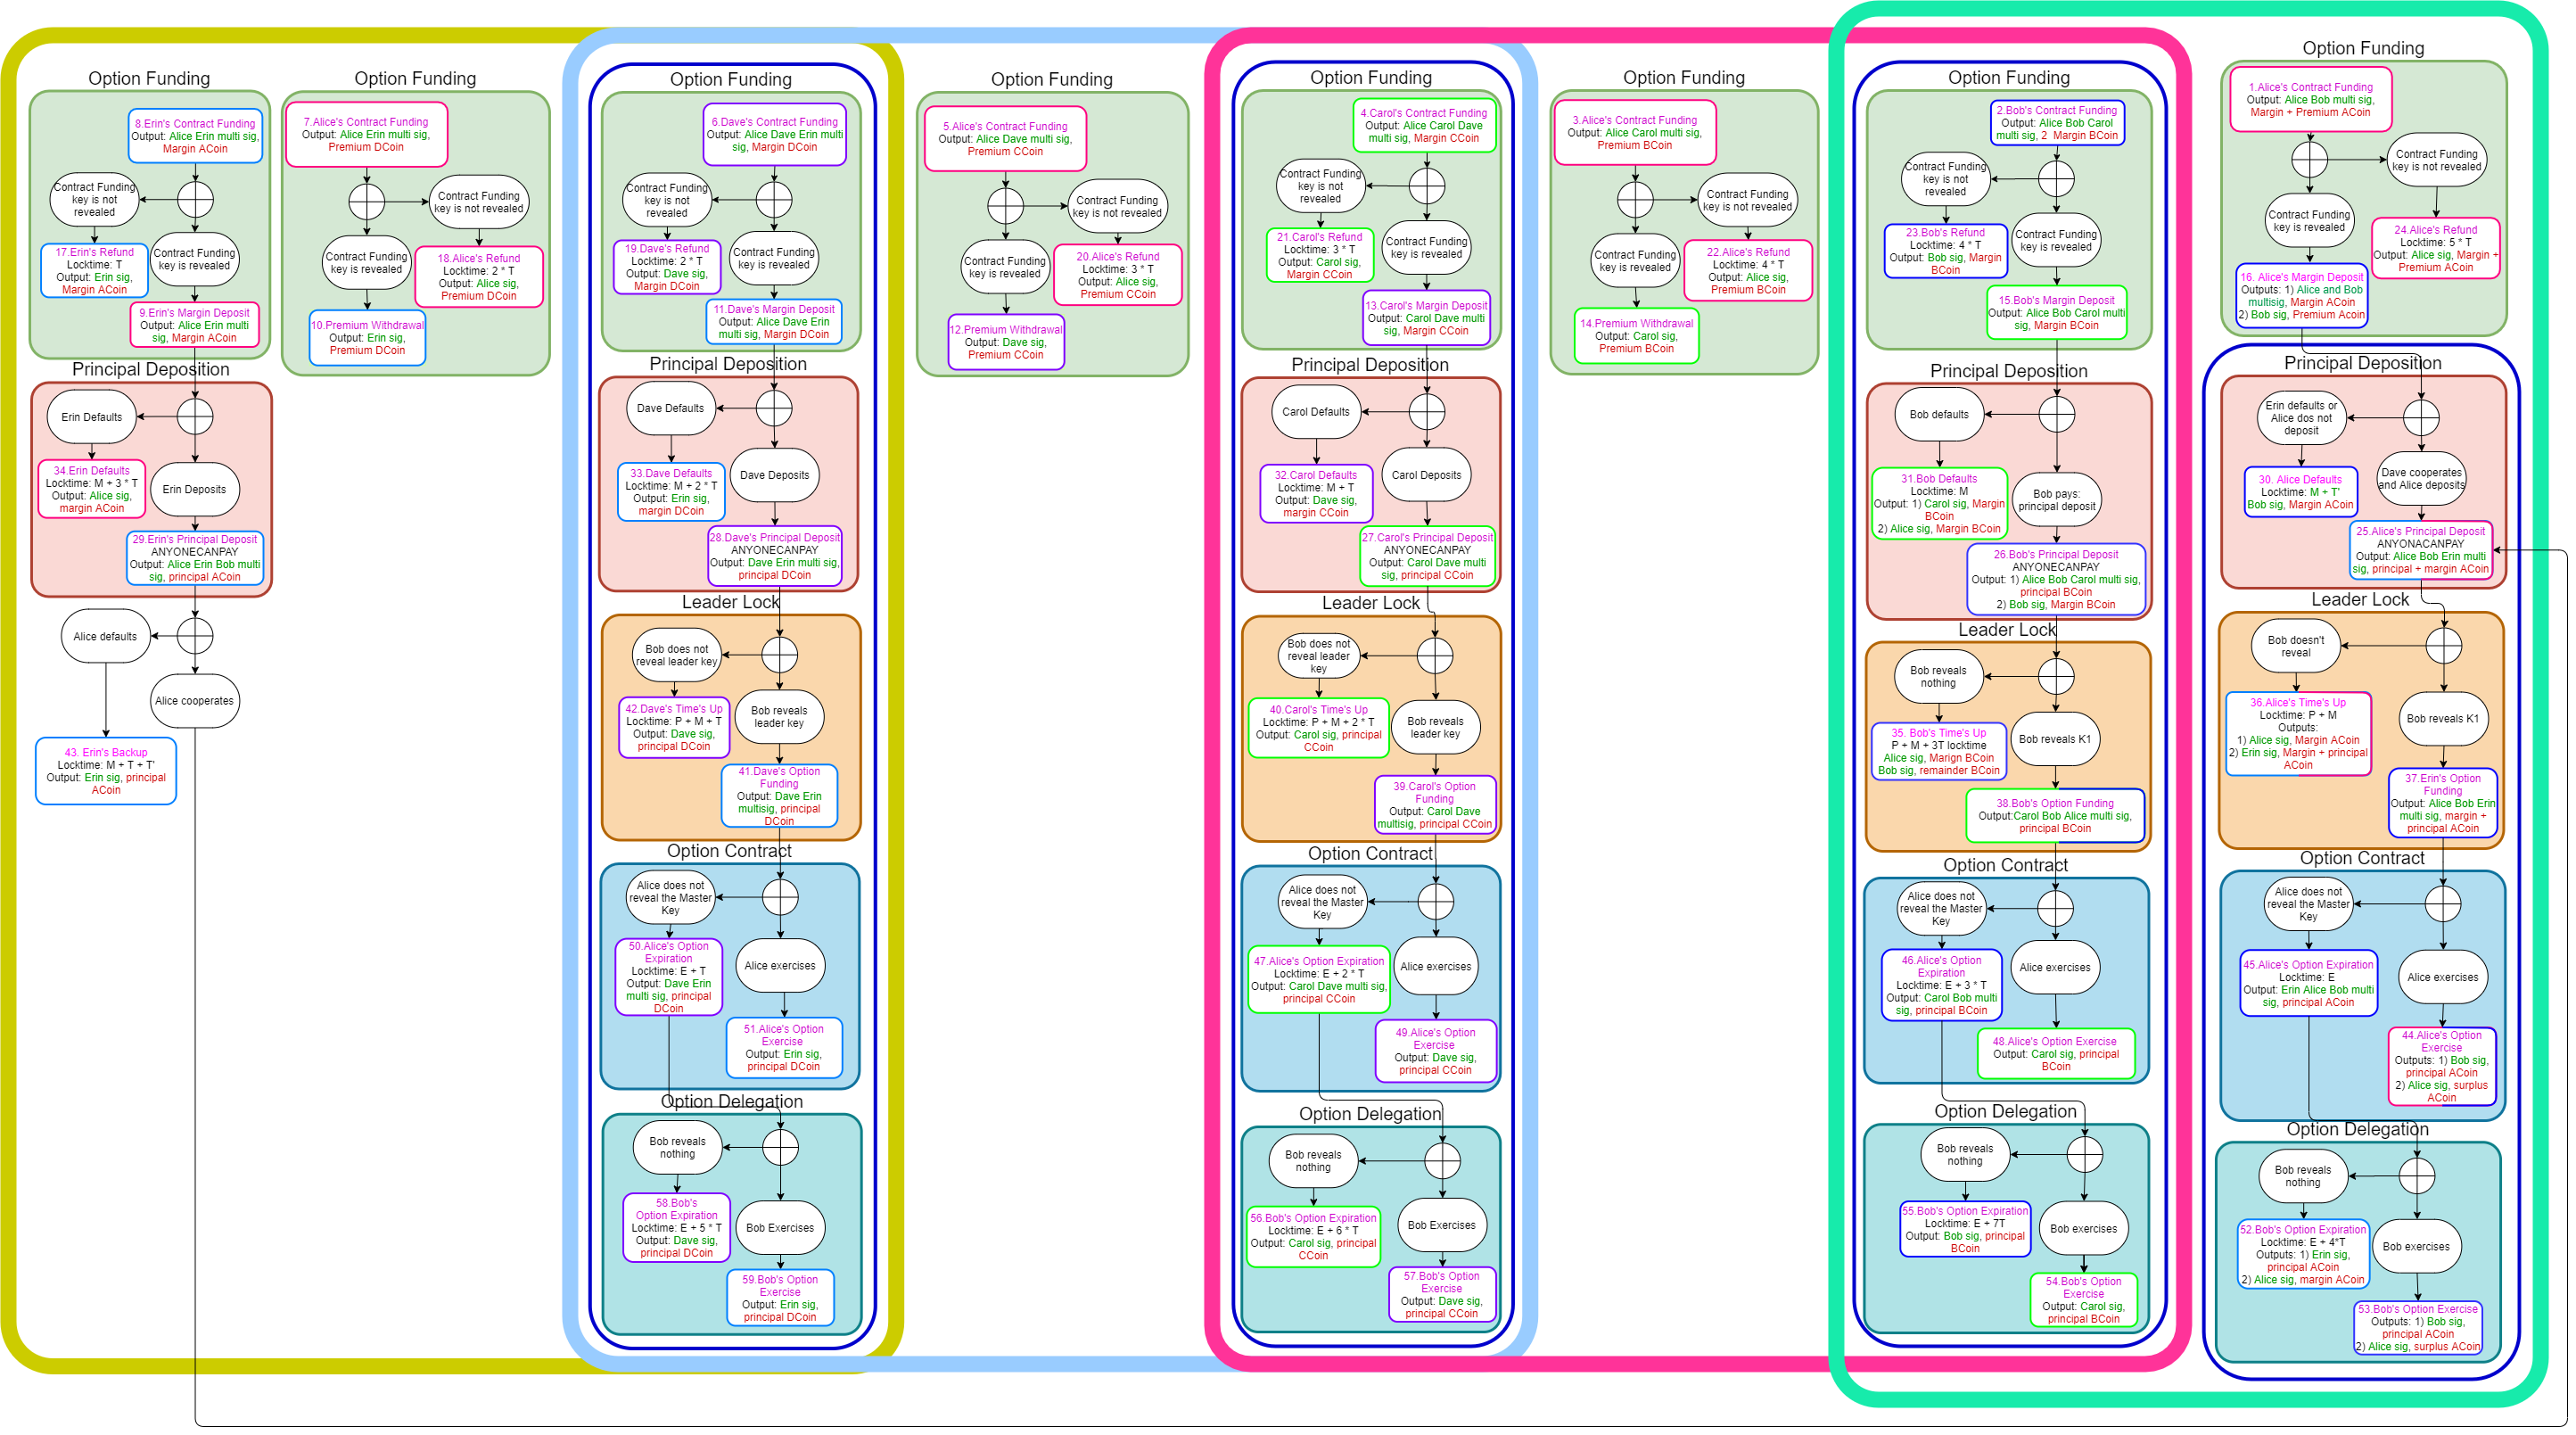
\includegraphics[width=\textwidth]{figures/arb_swaption.png}
%     \caption{The schematic for Margined Arbitrage}
%     \label{fig:margined_arg}
% \end{figure*}

% As mentioned earlier, Alice can use {\it Late Deposit} swaption as her first swaption in case she does not have all the principal at first. So, she only connects other parties to each other in a loop. Hence, there are four swaptions and Alice is not a party in any of them. She pays premium in any of them, though. She also has to deposit margin in the first swaption. Hence, the first swaption to start is the last swaption to finish and is between Erin and Bob. So, there are five margins and four swaptions. Alice's margin is only there to prevent her from cheating. The five phases of {\it Margined Arbitrage} are: 

% \begin{itemize}
%     \item \textbf{Contract Funding}: Similar to the lined arbitrage, every one has exchanged funding and refund transactions. Three types of these stages:
%     \begin{itemize}
%         \item Alice's first funding: includes margin + premium.
%         \item Other fundings of Alice: Only includes premium.
%         \item Bob's funding: includes margin which is worth twice other parties margins.
%         \item Other parties fundings: include only margin.
%     \end{itemize}
%     Alice reveals \Aone by broadcasting Erin's margin deposit transaction. Then Erin broadcasts Dave's margin deposit
%     transaction and everyone broadcasts the margin deposit transaction of their previous party. No one has the incentive not to broadcast this transaction since if they do not, they are the only one who goes through a loss. When all the 
%     margin deposit transactions are broadcast, the arbitrage goes to the next stage.
    
%     \item \textbf{Principal Deposition}: All swaptions except for the first one are {\it early deposit}, so the locktimes are ascending. On the other hand, the first swaption is a {\it late deposit}, so Alice's locktime has to be bigger than Bob's. Alice's principal is in fact a portion of the principal that Erin deposits. The swaption between Dave and Erin
%     is {\it early deposit}, so Erin's locktime has to be the biggest locktime. similar to the line arbitrage, if any one defaults
%     in this stage, and does not deposit their principal, the faulty party loses her margin (except for when it is Alice) and other parties
%     margins are exchanged counter clockwise. As mentioned earlier, the first swaption is between Erin and Bob, but Alice also puts margin to this swaption. The principal deposition of Erin is a ANYONECANPAY transaction. If she broadcasts it, Alice takes its output as an input to the principal deposit of the first swaption. We have given Erin a chance that if Alice did not do so, she can take her principal back and of course since Alice has defaulted she loses her margin. If everyone deposits their principal, we go to the next stage.
    
%     \item \textbf{Leader Lock}: Alice is waiting for Bob to reveal \keyone by broadcasting {\it Erin's Option Funding} transaction. If Bob does so, Erin broadcasts {\it Dave's Option Funding} transactions and 
%     every other party broadcasts the previous party's {\it Option Funding} transaction respectively. Timelock for Alice is the least and increased counter clockwise and Bob's the greates. {\it Bob's Option Function} transaction can be broadcast by both Carol and Bob. Otherwise other parties can collude 
%     and cheat on Bob using this attack: Bob reveals \keyone and others do not broadcast the {\it Option Funding} and take Bob's margin. Hence, when Bob can
%     broadcast his own option funding, there would not be any problem of this kind. 
    
%     Thus, if Bob reveals, every other party goes to the next stage. If Bob does not reveal \keyone, he loses his margin. If Bob reveals \keyone after P + M, Alice will immediately reveal \Atwo and Carol takes Bob's money. 
    
%     \item \textbf{Option Funding}: This is time for Alice to use her option.  She can reveal \Atwo by broadcasting the {\it 44.Alice's Option Exercise}. She takes her surplus and Bob gets his Acoins. She has to reveal it within E locktime. Since in all swpations the right-hand side party is in charge of revealing \Atwo the locktimes have to be descending. This means Alice's timelock has to be both greater and lower than Carol's. This is obviously
%     impossible. Hence, we set the timelocks so that Carol's locktime is greater than Alice's, which makes it possible for Carol and Alice to cheat on Bob, but we solve this problem using the \textbf{delegation stage}. Now consider that if Alice exercises her option till E locktime, then every party can take their new coins.
%     If Alice does not exercise till E, her option is delegated to Bob.
    
%     \item \textbf{Option Delegation}: If Alice has not exercised till E, Bob broadcasts the {\it Alice's Option Expiration} transactions number 45 and 46 and all other parties do the same (since it is their only chance 
%     to get their coins). Now the arbitrage is in the delegation stage. The option is now Bob's and everyone is waiting for him. If he decides to exercise, every one gets their new coins, otherwise every one gets their old coins. The timelocks are descending for all swaptions except the first one and in the first one they are ascending (like last stages). \fatemeC{The most important consideration is that if Alice has decided not to exercise her option, Bob would also not exercise. Since if it was not beneficial for Alice it would not be beneficial for Bob neither. the reason is that the coins that Alice gets are the same as Bob gets, so if one has lost its value the other one has lost too.(why the hell????)}
 
% \end{itemize}

% \begin{table*}[]
%     \centering
%     \begin{tabular}{|c|c|c|c|}
%     \hline
%         {\normalsize Stage} & {\normalsize LT in column 1} & {\normalsize LT in column 2i} & {\normalsize column 2i + 1}\\
%         \hline
        
%         {\normalsize Contract Funding} &
%         {\normalsize (n + 1)T} &
%         {\normalsize (N - i + 1)T} &
%         {\normalsize (N - i + 1)T} \\
        
%         {\normalsize Principal Deposition} &
%         {\normalsize $M + T'$} &
%         {\normalsize M + (N - i)T} & - \\
        
%         {\normalsize Leader Lock} & {\normalsize P + M} &
%         {\normalsize P + M + iT} & - \\
        
%         {\normalsize Option Contract} & 
%         {\normalsize E} &
%         {\normalsize E + (N - i)T} & - \\
        
%         {\normalsize Option Delegation} & 
%         {\normalsize E + NT} & 
%         {\normalsize E + (2N - i)T} & - \\
%         \hline
%     \end{tabular}
%     \caption{Locktimes for general case in an arbitrage. Each column in the table shows one column in the arbitrage.}
%     \label{tab:arb}
% \end{table*}

% Now consider the general case for the arbitrage when there are N swaptions.
% Table \ref{tab:arb} shows locktimes for each stage in a general arbitrage.
% Each column in the table shows one column in the arbitrage. Moreover, for simplicity we put locktimes so that different stages do not have overlap in time. In some cases stages overlapping can cause trouble. Two examples are: 

% \begin{itemize}
%     \item M has to be larger than (N + 1)T. Otherwise, Alice and Carol can broadcast the {\it Bob Defaults} transaction and then broadcast the {\it Alice's Refund} and take Bob's margins.
    
%     \item In the third stage, P + (N - 1)T has to be greater than $T'$. Otherwise, Alice can wait till P + M + (N - 1)T not deposition principal, then Bob has to broadcast the {\it Bob's Time's Up} and then Alice will deposit and then broadcast the {\it Alice's time's Up}. So, she takes Bob's margin without loosing any thing but premium.
% \end{itemize}


% Note that Alice in fact has E time to use her option. Then Bob takes the option, so we can say that Alice does not have any option but it is not true for two reasons: 1) Arbitrages are always zero-risk. 2) If she deposits her principal it means that all the parties have cooperated (if one does hot, she does not deposit principal and does not lose any thing, just the margins are exchanged which is inevitable). when all parties have cooperated and arbitrage is zero-risk every thing is fine so why would Alice not exercise?

% Note that when Alice is always going to use her option, so Alice is not in fact delegating her option to Bob, but by having the delegation stage, she only assures Bob that he would not be cheated.





% \section{comments}

%  \ahC{Time Elapsed Experiment.}\\
% \ahC{Reconstruction impossibility}\\
% \fatemeC{Is it reasonable to remove Option parts from Arbitrage. Arbitrages have absolute benefit in a short time, so the option is not needed to be given to Alice. However she can have it by adding the rest of the transactions.}\\
% \fatemeC{In section of tangle, mention that the algorithm may divide a line into many strongly connected parts. mention that it does not make any problem.}
% \ahC{Somewhere we have to mention the Option Delegation component can solve the multi leader problem. Yes in tangle. why the hell is this comment here?}
